% This template was initially provided by Dulip Withanage.
% Modifications for the database systems research group
% were made by Conny Junghans,  Jannik Strötgen and Michael Gertz

\documentclass[
     12pt,         % font size
     a4paper,      % paper format
     BCOR10mm,     % binding correction
     DIV14,        % stripe size for margin calculation
     ]{article}

%%%%%%%%%%%%%%%%%%%%%%%%%%%%%%%%%%%%%%%%%%%%%%%%%%%%%%%%%%%%

% PACKAGES:

% Use German :
\usepackage[english]{babel}
% Input and font encoding
\usepackage[latin1]{inputenc}
\usepackage[T1]{fontenc}
% Index-generation
\usepackage{makeidx}
% Einbinden von URLs:
\usepackage{url}
% Special \LaTex symbols (e.g. \BibTeX):
%\usepackage{doc}
% Include Graphic-files:
\usepackage{graphicx}
% Include doc++ generated tex-files:
%\usepackage{docxx}

% Fuer anderthalbzeiligen Textsatz
\usepackage{setspace}

% Fuer research questions
\usepackage{enumitem}

\usepackage{tabularx}
\usepackage{comment}

\newlist{questions}{enumerate}{2}
\setlist[questions,1]{label=RQ\arabic*.,ref=RQ\arabic*}
\setlist[questions,2]{label=(\alph*),ref=\thequestionsi(\alph*)}

% hyperrefs in the documents
 \PassOptionsToPackage{hyphens}{url}\usepackage[bookmarks=true,colorlinks,pdfpagelabels,pdfstartview = FitH,bookmarksopen = true,bookmarksnumbered = true,linkcolor = black,plainpages = false,hypertexnames = false,citecolor = black,urlcolor=black]{hyperref}
 \usepackage{hyperref}
 \def\UrlBreaks{\do\/\do-}
%%%%%%%%%%%%%%%%%%%%%%%%%%%%%%%%%%%%%%%%%%%%%%%%%%%%%%%%%%%%

% OTHER SETTINGS:

% Choose language
\newcommand{\setlang}[1]{\selectlanguage{#1}\nonfrenchspacing}


\begin{document}

% TITLE:
\pagenumbering{roman} 
\begin{titlepage}


\begin{center}
\vspace*{2cm}
\textbf{ 
\Large Heidelberg University\\
\smallskip
\Large Institute of Computer Science\\
%\smallskip
%\Large Database Systems Research Group\\
\smallskip
}

\vspace{3cm}

\textbf{\large Project Report for the lecture \\  Data Science for Text Analytics}

\vspace{0.5\baselineskip}
{\huge
\textbf{Hate, Discrimination \& Racism in German Rap - A Text Analytics Approach}
}
\end{center}

\vfill 

{\large
\begin{tabular}[l]{ll}
Johannes Sindlinger: & 3729339, Computer and Data Science, M. Sc.\\
  & johannes.sindlinger@stud.uni-heidelberg.de\\
Gal Lebel: & 3679087, Computer Science, B. Sc. \\
  & gal.lebel@stud.uni-heidelberg.de\\
  
\end{tabular}
}

\vspace{1cm}
\begin{tabular}[l]{ll}
Github-Repository: & \url{https://github.com/gsindlinger/IDSTA-Text-Miners} \\
Dataset: & Song Lyrics via Spotify API \& Genius \cite{genius} (see description below) \\
Advisor: & Nicolas Reuter
\end{tabular}
\end{titlepage}

\pagenumbering{arabic} 

\section*{Abstract}\label{sec:abstract}
The abstract is supposed to summarize your work in less than 300 words. It motivates your work, states the
problem, and highlights your project's main contributions. The abstract serves as a short summary for the
reader.

\section{Introduction}\label{sec:motivation}
'I leave no whore daughter unfucked, everyone wants my dick - even lesbians get turned around!' - Excerpts from song lines by German rappers such as Bausa \cite{steffes-lay_2019} provide material for discussion in German society and pose the question of how far artistic freedom can go in music and where insurmountable boundaries are crossed. Whether homophobia \cite{steffes-lay_2019}, misogyny \cite{steffes-lay_2019} or antisemitism \cite{salomo_greven_2021}, in the public perception German rap seems to be one thing above all: Harsh and unfair. The popularity and sales figures of German rappers, on the other hand, justify their song texts and acting: at the end of October 2022, there were a total of ten titles in the top 20 singles charts in Germany that can be assigned to the genre of German rap \cite{mtv_germany_2022}. And in 2021, rapper Capital Bra was the most successful German musician in terms of the number of different number 1 hits \cite{br_2019}. 

Contrary to the general negative impression, there are many attempts by artists who oppose against the negative image of rap in Germany with their lyrics and actions \cite{Deutschlandfunk_2021}. Some artists use their songs also used to specifically address sociopolitical issues - such as the 'Black Lives Matter' movement, police violence or the integration of refugees \cite{me-redaktion_2021}.

In this project, we would like to investigate the controversial debate around German Rap in an analytical manner. For this purpose, the song lyrics of various successful rappers of the genre of German rap will be analyzed on the basis of methods of textual data science. The following questions are the focus of our studies:

\begin{questions}
    \item \textbf{Do song lyrics of German rap in general possess a negative sentiment?}
    \item \textbf{Does hate, discrimination \& racism exist in German rap song lyrics?}
    \item \textbf{How prevalent is hate, discrimination \& racism in German rap song lyrics?}
\end{questions}

Detailed ideas to answer these questions, including the data pipeline which we want to use, are described in \autoref{sec:project}. Before that, the project will first be put into the context of existing literature in \autoref{sec:research}.












\section{Related Work}\label{sec:research}

Various journalistic and social science works in the past have dealt with the role of German rap in society as work from Lena Gauer \cite{gauer}, Melanie Heinisch \cite{heinisch}, Markus Klein \cite{klein2011dies} or Tobias Wiese \cite{wiese2021identitat}. 

Michael Huber \cite{wiegangsta} explains the popularity of the rap genre in the context of the rise 'Gangsta Rap', which finds its origin in the United States. According to Huber, 'Gangsta Rap' in Germany usually focuses on the so-called prison culture. In the lyrics of such songs, one very often encounters terms that deal with violence, drugs, separation from other social groups. It also conveys the hardships of being a minority in Germany and focuses on the socially weaker.

In addition to sociotechnical analyses, there are two data-driven approaches to analyze the song lyrics of various German rappers. In 2016, Bayerischer Rundfunk's cultural magazine Puls \cite{puls_2016} examined the political correctness of various song lyrics by German rappers, using a very similar methodology to the one we will use in this paper. Puls selected the five most commercially successful albums by German rappers in each year for the period 2006 to 2016 and downloaded the song lyrics via Genius. These song lyrics were examined for specific discriminatory word groups - with a particular focus on homophobic, racist, misogynistic, and ableist terms.

Puls observed that the use of discriminatory language increased over the first part of the sample period and decreased towards the end. Misogynistic and homophobic remarks played a particularly significant role. Discrimination against the disabled was also a permanent feature of the song lyrics studied, while racism was rather less prevalent. The author of the study also emphasizes the lower significance of the study due to the limitation to five albums per year.

Another quantitative analysis of the situation in Deutschrap is provided by Spiegel magazine \cite{rohwer_2020} in 2020. Author Bj{\"o}rn Rohwer concludes the following: The beginning of the 2000s marks a significant increase in the amount of German rap texts containing vulgarity, misogyny, sexism, anti-Semitism and violence. From about 4-5\% of German rap songs containing sexist terms, the 2000s marked a jump towards ca. 25\% of the songs containing such terms. Between 2005 and 2013 the trend has declined only to later on in 2018 go up again. An explanation for this might be, that sexism in rap songs has become more subtle by using less sexist terms but at the same time they still promote the sexist image and is also harder to detect by listeners as much as by means of text analysis.

In contrast to the analyses of Puls and Spiegel, we wanted to get a broader view of the sentiment of German rap. Concretely, we did not only consider frequencies of certain words, but more in-depth methods of text analysis, which are based on machine learning. In addition to that, we also included data from more artists and songs in our analysis compared to Puls. Generally, the goal of this project was to gain as much information as possible about song lyrics and to determine their 'fairness' in social context.














\section{Methods}\label{sec:project}

As already outlined in \autoref{sec:motivation}, this project will study the extent to which hate, discrimination, and racism influence German rap. For this purpose, we would like to use different methods of text analysis, which will be explained in more detail below. The described approach will also be supplemented by a visual representation in \autoref{fig:pipeline}.

\begin{figure}[!htb]
  \centering
  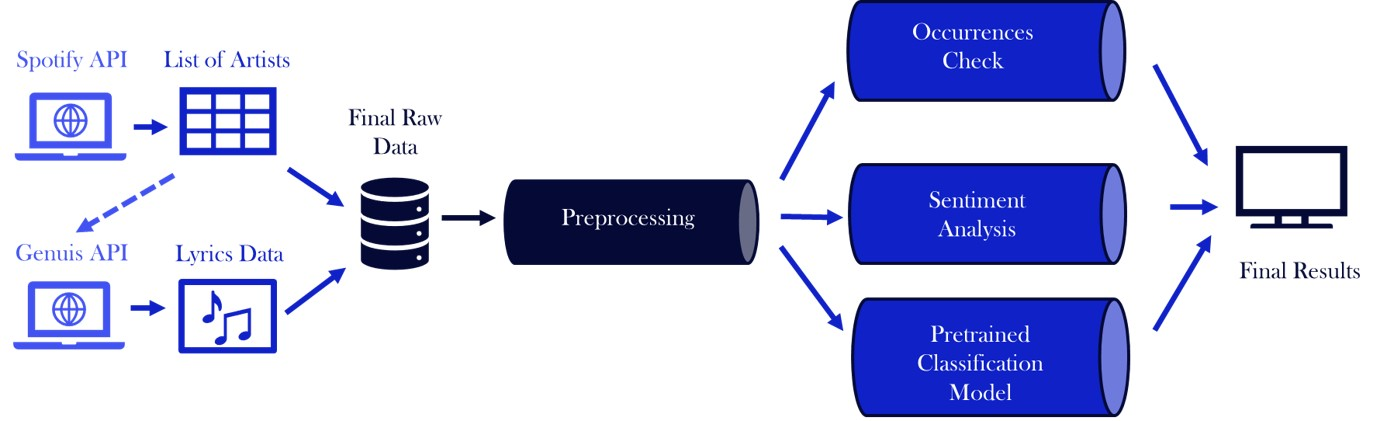
\includegraphics[width=\textwidth]{figures/pipeline.jpg}
  \caption[]{Text Analytics Pipeline}
  \label{fig:pipeline}
  \end{figure}

  \begin{itemize}
    \item Data
    \item Preprocessing
    \item Occurrences check
    \item Sentiment analysis
    \item Toxicity analysis
    \item Zero-shot classifier
\end{itemize}

As a basis for our investigations, a data set on certain artists of the German Rap will be used, which is not finally defined yet. This will be done in the nearest future using information from the web in manual and partially automated work. Corresponding information about artists can be extracted, for example, from \cite{last.fm,tonspion_2021}. The names of those artists are used in a further step to download the lyrics of all songs of those artists via the song lyrics platform Genius \cite{genius}. Genius is an online database for any kind of artistic texts and offers an API interface that provides license-free lyrics of many song lyrics. Since Genius does not fully provide all the data of every international artist, it might be necessary to accept limitations for some artists.

The song lyrics, enriched with information about the artists themselves, finally form the basis of our textual analyses: Since we would like to use pretrained models for the analysis of the lyrics in a further step and many of these models only support English-language texts, it might be necessary to translate the German song lyrics first. For this, we intend to use the Python framework DL Translate \cite{lu_2022}, since it is the only package that can freely translate unlimited texts. The translated lyrics, will be stored together with the original lyrics in ElasticSearch. It must be taken into account that by using such a translation tool, possible linguistic-relevant contexts will be incorrectly transferred into the English language. However, since there is considerable interpretative space in the context of song lyrics, this limitation should not be of too much importance. In fact, it is important to keep in mind for the entire project that the song lyrics studied allow for different interpretations, which can only be determined by machine analysis to a limited extent.

As indicated in the paragraph before, we would like to store the translated song lyrics together with the original data in ElasticSearch. The possibilities that ElasticSearch offers in the area of tokenization, classification of words including counting of word frequencies, etc. shall then be used as a basis for a first analysis of the song lyrics.

In addition to the described methods offered by ElasticSearch, we would like to use predefined machine learning models to enrich the data of the song lyrics. In this context, the frameworks used should be considered as a black box, and the corresponding methods remain untouched. We will consider the following frameworks:

The project Deep Learning Models for Multilingual Hate Speech Detection \cite{deepMLhatespeech} includes multiple models that can be trained or fine-tuned for recognizing hate speech in various languages, especially German. Performing hate detection using different machine learning algorithms in parallel would enable a more thorough analysis of the texts like: highlighting songs that get a high hate rate from most models, identifying common patterns between such songs and classifying them into subclasses according to the target of the hate speech (foreigners, women, disabled people etc.).

The German Sentiment classification with BERT \cite{guhr2020training} is a sentiment classification model trained on around 1.8 million German-language text samples coming from various sources (social media, movie, app and hotel reviews). It could be a starting point for identifying potential hateful song lyrics. Given the three sentiment classes used by this model (negative, neutral and positive), we could filter out texts classified as positive and also separate negative from neutral lyrics for the upcoming pipeline stages.

NLTK.Vader \cite{vader} is an NLP algorithm trained for performing sentiment analysis. It is best suited for short texts like posts on social media, containing some slang and abbreviations. Hence, our dataset on German song lyrics would make a good fit for this model (providing we first use a translation model like mBart \cite{mBart}).

HateSonar \cite{davidson2017automated} is a BERT based model built with Python for hate speech detection. It only works with English data, therefore the German song lyrics would first need to be translated. As with models trained on German texts, it would be beneficial to the analysis to extract information regarding hate speech from multiple models.

If there is time left, we would like to develop independent machine learning models on our own using the methods discussed in the lecture. However, this requires classification of the existing lyrics data, which would likely need to be done manually. Furthermore, the amount of data available could prove challenging with this approach. If it is not feasible to identify a very large number of song lyrics using the listed approach above, it could be difficult to develop meaningful machine learning models.

Finally, the results of the different analysis methods will be interpreted and visualized. Thereby, the findings of the analyses shall be explicitly highlighted using the lyrics data by visual markers. Additionally, results of the different metrics will be displayed. 

\section{Results}\label{sec:results}

As described in \autoref{sec:project}, the data of 5992 songs by German rap artists formed the basis of our research. For each song, information on the artists contributing, the album and the date of release was stored. This information was obtained using the Genius API. In addition, the final data set contains the lyrics to the corresponding song, which were treated using the preprocessing procedure described above and also saved in modified form.

The 5992 songs that remained after discarding non-German songs include 2094 participating artists and are spread among 1711 different albums. The number of artists involved includes not only primary artists, but also producers and featured artists. For example, the two producers Tim Wilke and David Kraft are the most frequent artists with 68 occurrences in the 5992 songs. The third most frequent artist in the available lyrics is Sido with 65 occurrences.

888 songs were declared as singles by Genius and were therefore not assigned to an album. This class also forms by far the largest share of the existing albums. The other existing albums are largely based on the limitation of song scraping to 15 songs per artist (see \autoref{sec:project}). The albums 'Instinkt' and 'Berlins Most Wanted' are both listed as 15 albums of one song. Only the album 'Liebeskummerparty' has 16 occurrences due to a song with a different artist.

\autoref{fig:number_songs} shows the temporal distribution of the songs. As it can be seen from the figure, the data set contains considerably fewer songs in the years 1998 to 2010 than in the period from 2010 to 2022. This could be due to the procedure for generating the data, which is essentially based on the predefined playlists from Spotify and the availability of various songs on the lyrics platform Genius. In addition, the number of artists in the Deutschrap genre has grown steadily over the years and was very low when the genre first emerged. The described disparity of the data affects the interpretability of the analyses. Details on this are explained in detail in the following sections.

\begin{figure}[!htb]
    \centering
    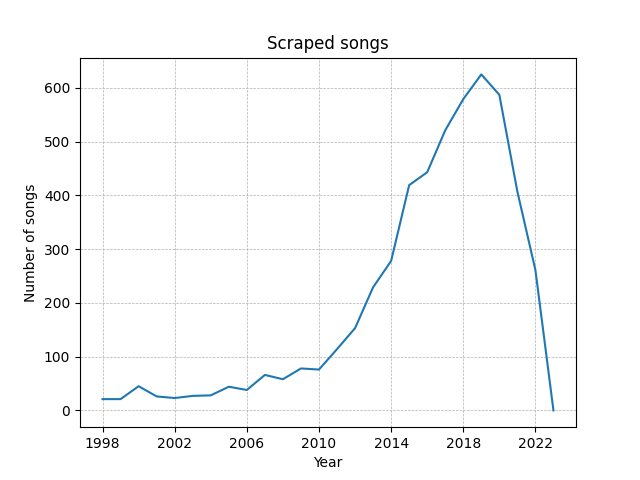
\includegraphics[width=0.8\textwidth]{figures/number_of_songs.png}
    \caption{Temporal distribution of scraped songs}
    \label{fig:number_songs}
\end{figure}

In the following, the results of the three different approaches to analyze the data will be presented in detail.

\subsection*{Occurrences check}

As outlined in \autoref*{sec:project}, an essential part of the task of the occurrences check was to elaborate a suitable dictionary for different categories, on the basis of which occurrences within the lyrics could be retrieved. After executing the process described in \autoref{sec:project} via Word2Vec and manual adjustment, the following quantities of words remained per category:

\def\arraystretch{1.2}
\begin{table}[!hbt]
    \centering
    \begin{tabular}{|l|l|}
    \hline
    \textbf{Category} & \textbf{Number of words} \\ \hline
    Misogyny        & 19 \\ \hline
    Violence        & 17 \\ \hline
    Anti-Semitism   & 14 \\ \hline
    Homophobia      & 14 \\ \hline
    Anti-disability & 13 \\ \hline
    Grief           & 12 \\ \hline
    Love            & 10 \\ \hline
    Racism          & 6  \\ \hline
    \end{tabular}
    \caption{Number of terms within each category of occurrences check}
    \label{tab:dictionary}
\end{table}

The different number of words per category is due to the fact that certain categories have fewer diverse terms than others. For example, the category misogyny contains a wide variety of vulgar terms for prostitutes, while the racism category almost exclusively contains the word 'nigger'.

The following \autoref{tab:occurrences_total} shows the absolute count of occurrences of the different categories in the entire data set. The categories love, misogyny and violence combine more than 85\% of all occurrences with 31451 of 36833 counted occurrences. 3628 of the examined songs contain at least one occurrence of the category love, which corresponds to about 61\% of the entire data set. The category violence was detected at least once in 3099 songs, approximately 52\% of all songs. We detected misogynistic terms in 2431 songs, about 41\% of the population. In 757 songs, no occurrences of the predefined categories could be found.

\begin{table}[!htb]
    \centering
    \begin{tabular}{|l|l|}
    \hline
    \textbf{Category} & \textbf{Number of occurrences} \\ \hline
    Love              & 12098                          \\ \hline
    Violence          & 10251                          \\ \hline
    Misogyny          & 9102                           \\ \hline
    Racism            & 2051                           \\ \hline
    Grief             & 1294                           \\ \hline
    Homophobia        & 1253                           \\ \hline
    Anti-disability   & 546                            \\ \hline
    Anti-semitism     & 238                            \\ \hline
    \end{tabular}
    \caption{Absolute count of occurrences of investigated categories}
    \label{tab:occurrences_total}
\end{table}

For further analysis, we examined the behaviour of the occurrences based on the release date of the songs. Due to the previously mentioned bias in the number of songs per year, we normalised the number of occurrences per year. \autoref{fig:occurrences_time_series} shows the development of the occurrences over the examined period 1998 to 2022. The different lines show the normalised number of occurrences per song for each category. The different categories are marked with different colours. It can be observed that especially around the year 2003, a relatively large number of songs contained violent and misogynistic terms, but at the same time also many on the subject of love. Until 2010, the occurrences of the three mentioned categories decrease to an average level of 3 occurrences per song. They maintain this level in the following years up to 2022. The other categories are less prevalent throughout the entire study period: Only the categories homophobia in 2006 and racism in 2003 exceed the mark of 1 average occurrence per song.

\begin{figure}[!htb]
    \centering
    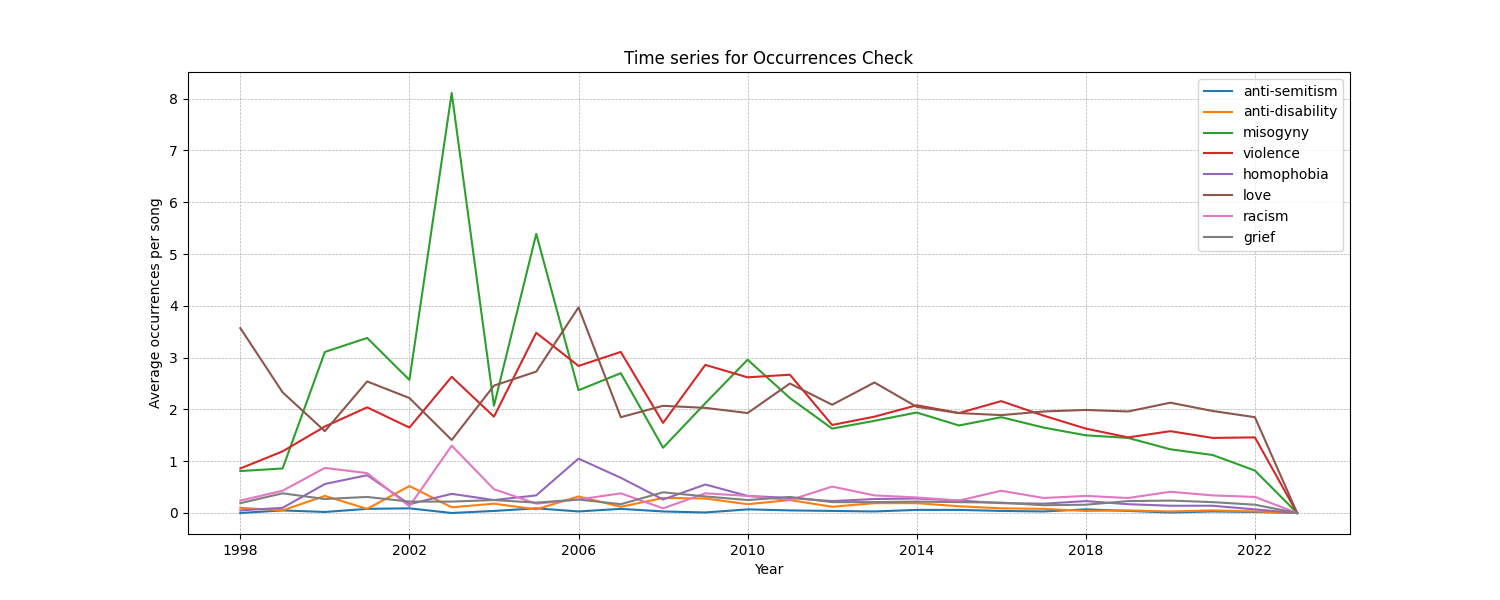
\includegraphics[width=\textwidth]{figures/time_series_occurrences.png}
    \caption{Time series analysis of counted occurrences}
    \label{fig:occurrences_time_series}
\end{figure}

\subsection*{Sentiment analysis}

For the analysis of the two described methods for sentiment analysis (German Sentiment Bert and Toxicity), we studied the distributions of the values across the data set. \autoref{fig:sentiment} shows the distribution of the values of the German-Sentiment-Model according to the described procedure in \autoref{sec:project}. Similarly, \autoref{fig:toxicity} shows the distributions of the values of the toxicity classifier. The left graph of the figure represents a histogram of the distribution over the complete investigation period. The right graph in contrast shows the temporal course of the values. The middle blue line within this graph corresponds to the median of the examined songs within each year, the surrounding shaded area contains all data that falls into the range of the 25\%- to 75\%-quantile. In other words, 50\% of the songs examined have a sentiment or toxicity value within the shaded area.

In general, one can observe for the sentiment analysis via German Sentiment Bert that a negative sentiment prevails in the songs. The median of all data is -0.40, the 25\% quantile is -0.52 and the 75\% quantile is -0.27. The clustering of data in this range can also be gathered from the histogram in \autoref{fig:sentiment}. Only 263 songs were assigned a sentiment greater than 0, which corresponds to a share of 4.4\% of all the songs examined. 

The time series analysis of the sentiment data on the right-hand side of \autoref{fig:sentiment} reveals no meaningful change in the sentiment of the songs studied over the research period. The median decreases slightly from -0.36 in 1998 to -0.42 in 2022. The lowest median can be found in 2009 with a value of -0.47, and the highest median in 2003 with a value of -0.31.

\begin{figure}[!htb]
    \centering
    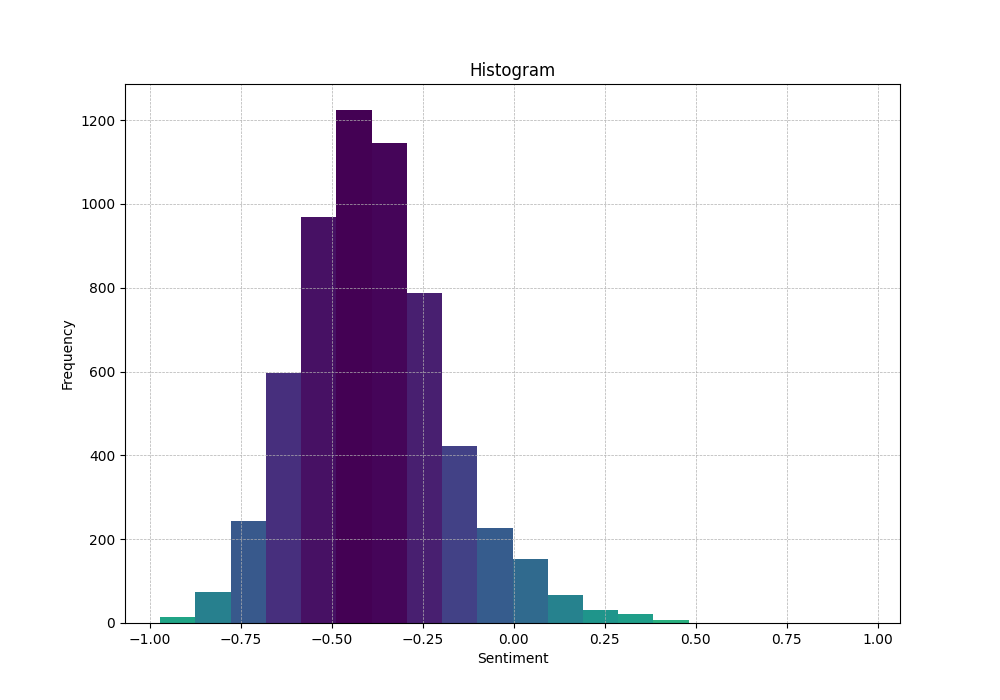
\includegraphics[width=0.49\textwidth]{figures/sentiment_histogram.png}
    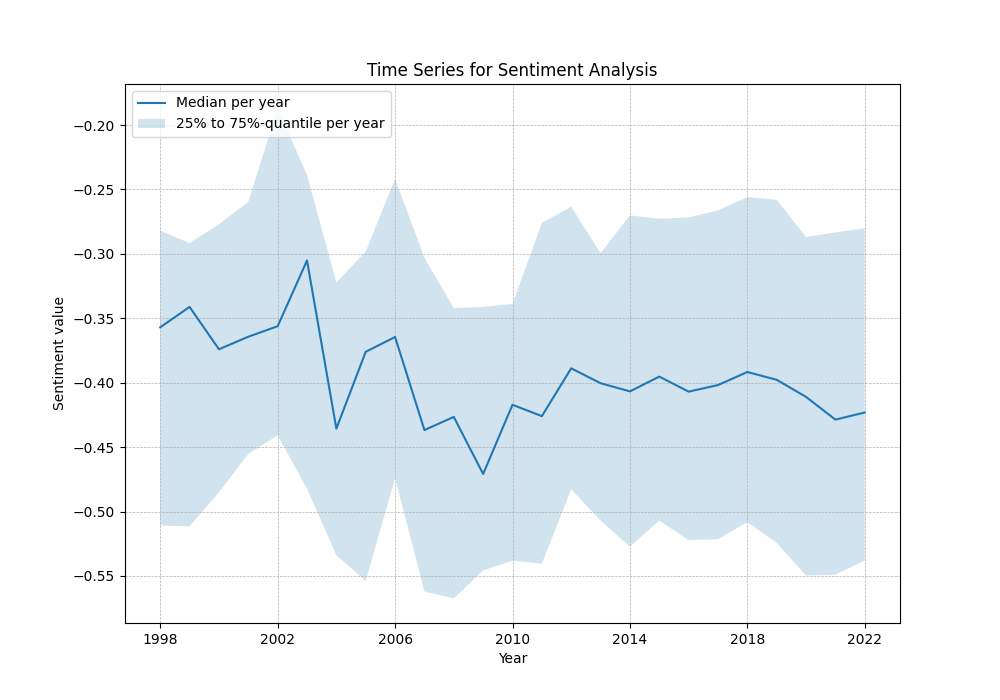
\includegraphics[width=0.49\textwidth]{figures/time_series_sentiment.png}
    \caption{Distribution of results regarding German-Bert-Sentiment analysis}
    \label{fig:sentiment}
\end{figure}

The toxicity analysis also shows a rather one-sided distribution of the examined data, as the histogram on the left side of \autoref{fig:toxicity} shows. 1100 songs are classified with a positive value by the toxicity classifier, i.e. they are classified as rather toxic. This corresponds to a share of 18\% of the population. The median of the toxicity values of all songs is -0.34, the 25\% quantile is -0.60 and the 75\% quantile is -0.08. The development over time, shown on the right side in \autoref{fig:toxicity}, shows a slight downward trend over the years. In other words, songs are becoming less toxic based on the toxicity analysis, but with the starting level in the 2000s already being classified as non-toxic.

\begin{figure}[!htb]
    \centering
    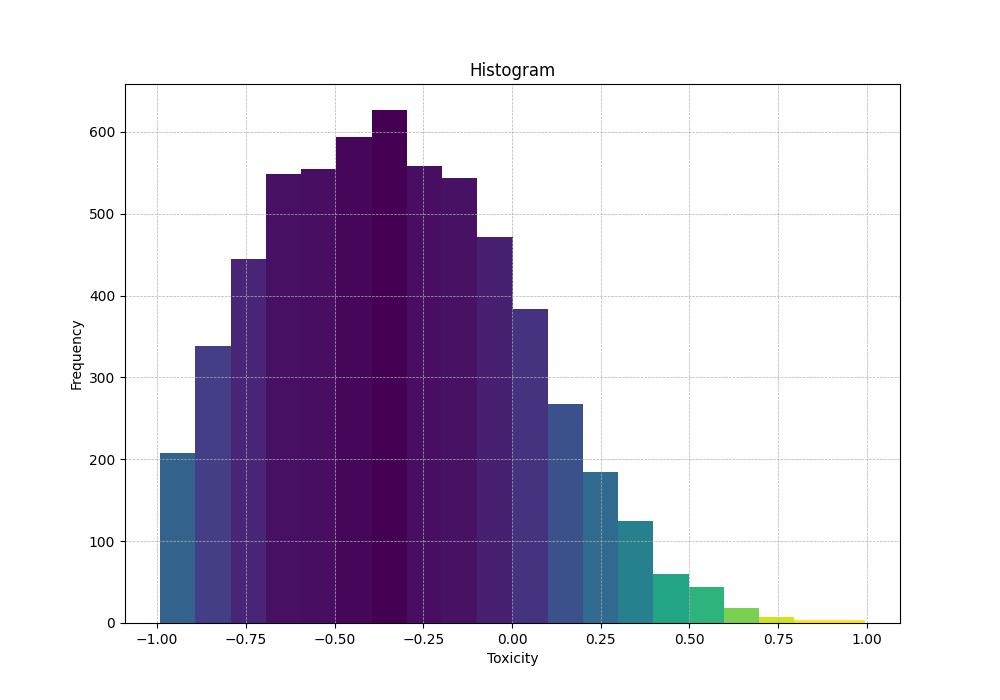
\includegraphics[width=0.49\textwidth]{figures/toxicity_histogram.png}
    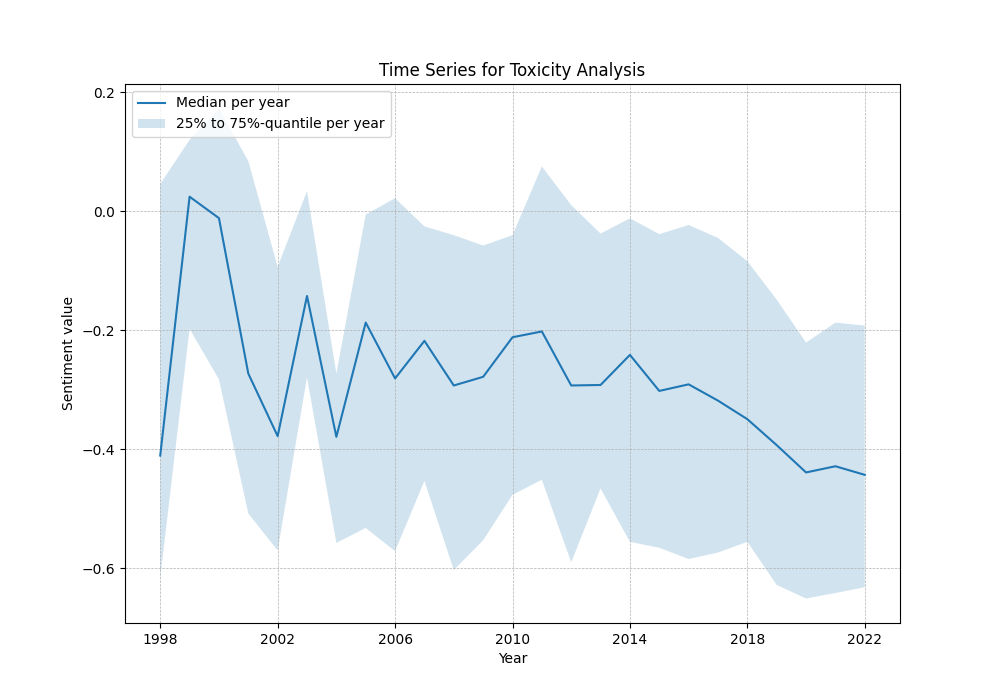
\includegraphics[width=0.49\textwidth]{figures/time_series_toxicity.png}
    \caption{Distribution of results regarding Toxicity analysis}
    \label{fig:toxicity}
\end{figure}

\subsection*{Zero-shot classifier}

The classification via zero-shot method (see \autoref{sec:project}) provides probabilities for the given classes per song. Figure \autoref{fig:zero-shot} shows the distribution of classes across the data set. The graph on the left only considers the most likely class per song and ignores all probabilities of the other classes. It thus corresponds to a one-hot-encoded classification to a single category per song. As one can see from the graph, the class 'positive' is the most prevalent with 2149 songs assigned to it, followed by the category 'friendly' with 1732 occurrences and 'violent' with 935 occurrences. The categories 'affectionate', 'neutral' and 'mysoginistic' were selected as the most likely category only a few times. 'Racist' and 'homophobic' were not assigned to any song with highest probability.

Looking at the left side of the \autoref{fig:zero-shot}, one gets insight into the summed probabilities of the categories. This reveals a slightly differentiated picture: The categories 'positive' and 'friendly' remain at the top, but with a smaller difference compared to the one-hot-encoded approach on the left side of \autoref{fig:zero-shot}. The categories 'affectionate', 'violent', 'neutral' and 'mysoginistic' gain more importance in this view. Racist' and 'homophobic' are still relatively underrepresented.


\begin{figure}[!htb]
    \centering
    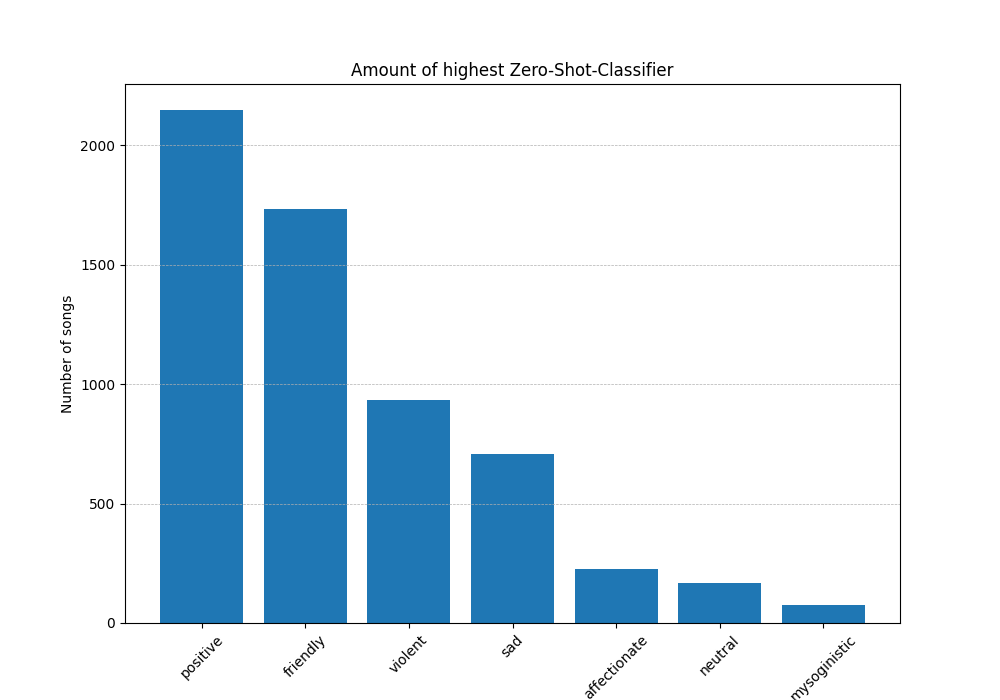
\includegraphics[width=0.49\textwidth]{figures/overall_score_binary_zero_shot.png}
    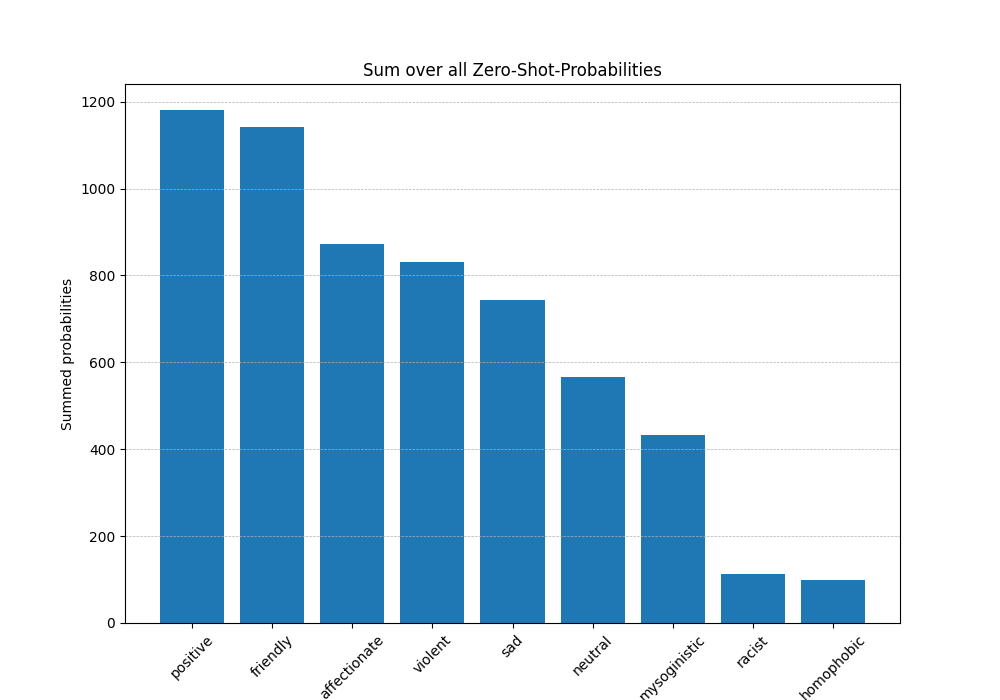
\includegraphics[width=0.49\textwidth]{figures/overall_score_zero_shot.png}
    \caption{Distribution of categories regarding zero-shot classifier}
    \label{fig:zero-shot}
\end{figure}

The following diagram in \autoref{fig:zero-shot2} provides an in-depth view of the development of the data over time with regard to the zero-shot classification: Four-year periods in the study period 1998 to 2022 are each shown with the three predominant categories in relation to the summed probabilities of the classifier. Due to the bias in the number of songs in the different periods (see \autoref{fig:number_songs}), the sum of the probabilities was divided by the number of songs per period. Over the period studied, the values of the two most probable categories 'friendly' and 'positive' are close to each other and continue to converge. Until 2014, the third most relevant category is 'violent', before it is replaced by 'affectionate'. The average probability for the third highest category is between 12.5\% and 15\%. 

\begin{figure}[!htb]
    \centering
    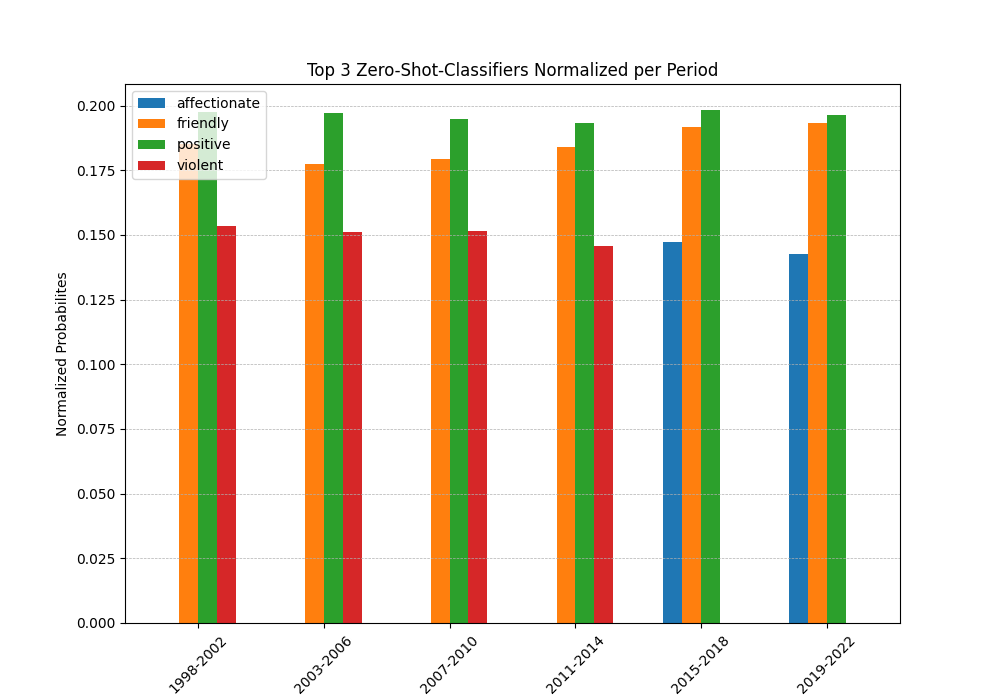
\includegraphics[width=\textwidth]{figures/top_3_time_series_zero_shot.png}
    \caption{Time series analysis for the top 3 prevalent categories of zero-shot-classifier}
    \label{fig:zero-shot2}
\end{figure}

\subsection*{Evaluation}

In order to be able to classify the results and assess their quality, we have developed methods for evaluating the results. No evaluation was carried out for the occurrence test, as this method is based on pure counting and therefore only allows for misinterpretation to a limited extent. For the other methods, we faced the challenge that the data used was not labelled as it should be for a complete evaluation. Our dataset was self-acquired, so we had no data against which to compare the results of our methods.

One of the options we considered at this stage was to use ChatGPT \ OpenAI's Playground platform to automate the very time-consuming process of labelling the songs. Unfortunately, we encountered a few problems in the process. One of them was the inconsistency of the labelling, i.e. the same lines were interpreted and classified differently each time they are given as input to the AI. However, this might be something a human could do as well, one could interpret things from different perspectives at different times. One even more majore issue was the recognition of swear words in OpenAI, of which there are many in German rap, which completely ruled out this option for us.


We therefore decided to manually label about 70 songs, of which we had an equal number from each classes of the three different methods used, so we were able to equally evaluate the efficiency and accuracy of the methods in relation to the different labels we had. During the labelling process, we realised how difficult it is even for people to assign a label, be it a positive, negative or even more specific label (like racist, misogynistic, etc.). Many biases could influence the decision, and the songs leave a lot of room for different perspectives and interpretations of their content. 

So the task of labeling the songs itself proved to be very challenging, which is why we decided not to give the chosen label a percentage probability, but to simply classify them in a binary way. So we decided to ignore the exact probabilities that the different methods assigned to the different possible classes and consider them as a binary classification.


For the evaluation, we've decided to use a Confusion Matrix and consider the F1 Score.
We've compared our labels with the predictions of the different methods in the following manner:
\begin{itemize}
    \item Sentiment Analysis (German Sentiment Bert): We mapped any negative sentiment, i.e. probability less than 0, to -1 and any positive sentiment to 1.
    \item Toxicity Analysis: We did the same approach as for German Sentiment Bert: Mapping was done to -1 for not toxic songs and 1 for toxic songs.
    \item Zero-shot Classification: We omitted the probabilities and took the class with the highest probability as the label of the song.
\end{itemize}

The confusion matrices for the different methods can be found below:

\begin{table}[!htb]
    \centering
    \begin{tabular}{l|llll}
     & Precision & Recall & F1-Score & support \\ \hline \hline
    negative & 0.98 & 0.63 & 0.77 & 65\\
    positive & 0.08 & 0.67 & 0.14 & 3 \\ \hline
    accuracy & & & 0.63 & 68\\
    macro avg & 0.53 & 0.65 & 0.45 & 68 \\
    weighted avg & 0.94 & 0.63 & 0.74 & 68\\
    \end{tabular}
    \caption{Confusion matrix for Sentiment Analysis (German Sentiment Bert)}
    \label{tab:confusion_matrix_sentiment}
\end{table}

\begin{table}[!htb]
    \centering
    \begin{tabular}{l|llll}
     & Precision & Recall & F1-Score & support \\ \hline \hline
    neutral & 1.00 & 0.53 & 0.69 & 66\\
    toxic & 0.06 & 1.00 & 0.11 & 2 \\ \hline
    accuracy & & & 0.54 & 68\\
    macro avg & 0.53 & 0.77 & 0.40 & 68 \\
    weighted avg & 0.97 & 0.54 & 0.68 & 68\\
    \end{tabular}
    \caption{Confusion matrix for Toxicity Analysis}
    \label{tab:confusion_matrix_toxicity}
\end{table}

\begin{table}[!htb]
\centering
\begin{tabular}{l|llll}
 & Precision & Recall & F1-Score & support \\ \hline \hline
neutral & 0.22 & 0.22 & 0.22 & 9\\
affectionate & 0.78 & 0.70 & 0.74 & 10 \\ 
violent & 0.40 & 0.67 & 0.50 & 0.9\\
racist & 0.00 & 0.00 & 0.00 & 0\\
homophobic & 0.00 & 0.00 & 0.00 & 0\\
misogynist & 0.60 & 0.33 & 0.43 & 9\\
friendly & 0.00 & 0.00 & 0.00 & 10\\
positive & 0.50 & 0.36 & 0.42 & 11\\
sad & 0.48 & 1.00 & 0.65 & 10\\ \hline
accuracy & & & 0.47 & 68\\
macro avg & 0.37 & 0.41 & 0.37 & 68 \\
weighted avg & 0.43 & 0.47 & 0.42 & 68\\
\end{tabular}
\caption{Confusion matrix for Zero-shot Classifier}
\label{tab:confusion_matrix_zero_shot}
\end{table}









\section{Analysis}\label{sec:analysis}

Lorem ipsum

\section{Conclusion}\label{sec:conclusion}

To conclude, we will answer the initial research questions based on the analyses presented above and discuss some limitations and problems of our project.

\begin{questions}
    \item \textbf{Do song lyrics of German rap in general possess a negative sentiment?} \\
    Due to the limited evaluation results of the pre-trained models (German Sentiment Bert, Toxicity, Zero-shot Classification), the question whether a negative sentiment generally prevails in German rap can only be adequately answered based on the occurrences check. However, for the occurrences check, it can be stated that a general negative sentiment does not necessarily apply to the songs of the German raps. The comparison of the three most prevalent categories love, violence and misogyny in the occurrences check shows that all three categories have comparatively high occurrences in the lyrics, so the category love represents an opposition to the others. 
    \item \textbf{Does hate, discrimination \& racism exist in German rap song lyrics?} \\
    All four different methods of our analysis indicate the actual presence of hateful, discriminatory and racist topics in the lyrics. In particular, the occurrences check shows high occurrences of the categories violence and misogyny, the pre-trained models underline this assumption either. However, it should be noted that the evaluation of these models was weak.
    \item \textbf{How prevalent is hate, discrimination \& racism in German rap song lyrics?} \\
    A precise quantification of the presence of negatively associated topics in German rap songs is difficult on the basis of the research carried out. However, the occurrences check shows that about 50\% of German rap songs contain themes of violence, about 41\% themes of misogyny (see \autoref{sec:results}). Over time, it seems that violence, discrimination and racism play a decreasing role in German rap.
\end{questions}

During our work on the project, we encountered several difficulties that limited our ability to work on the songs correctly.

One of the main problems we encountered was the way the lyrics are written. The language used in German rap is special: slang, juvenile words, foreign words and the phonetic way of writing and spelling lyrics characterise this genre. All this made the pre-processing of these texts difficult using natural language processing tools such as lemmatisation and tokenisation. 

As an example, many words are written as they are spoken, i.e. 'ich hab' statt 'ich habe'. Another example is the word 'eine', which is often written as 'ne'. In other cases, nouns were not written with a capital letter, which made it difficult to distinguish between a verb and a noun.  Because of these deviations from the correct spelling of words, lemmatisation or stop word removal does not work, i.e. the word 'ne' wouldn't be removed because it is not recognised as a stop word. We tried to overcome this issue by using regex, but it was impossible to account for all cases. In our experiments, we found that words that were not supposed to be affected by the various regex rules were changed etiher, making this option useless. This limitation eventually made it impossible to learn the vocabulary of these songs with methods like Word2Vec accurately. The same words were treated as two different words depending on how they were spelled, i.e. 'hab' and 'habe' were considered as two different words.

A further difficulty that may have limited our results even more was the lack of punctuation. For correct processing of the texts, whole songs should be correctly divided into different sentences. The lack of punctuation in most of the songs prevented us from understanding which word belonged to which part of the lyrics. We were able to solve this problem with the automatic punctuation model mentioned in the pipeline section. Without this solution, it would have been very difficult to process the songs, even with pre-trained models.

The biggest lesson we learnt from this project, due to the mentioned limitations and the resulting weaknesses in the results, is that the quality of the data is of vital importance for the success of a text analytics project. 

\newpage


\bibliographystyle{plain}
% b) The File:
\bibliography{references}

\thispagestyle{empty}
\newpage
\section*{}
\begin{center}
\large\textbf Project contributions \\
\normalsize Incl. former team members Mara-Eliana Popescu and Simon K{\"o}rner
\end{center}

\vspace*{1cm}

\begin{table}[!ht]
    \centering
    \begin{tabularx}{\textwidth}{|l|p{4cm}|X|}
    \hline
        \textbf{Date} & \textbf{Who?} & \textbf{What?} \\ \hline
        Oct 28 & Johannes Sindlinger & Design pipeline graphics \\ \hline
        Oct 28 & Johannes Sindlinger & Write motivation, research topic (partly), project description (partly) \\ \hline
        Oct 30 & Mara-Eliana Popescu & Extend project description \\ \hline
        Oct 31 & Gal Lebel & Extend research topic, finish proposal \\ \hline
        Nov 18 & Johannes Sindlinger & Setup issues for project start \\ \hline
        Nov 25 & Johannes Sindlinger & Create artist list via Spotify API \\ \hline
        Dec 10 & Gal Lebel & Genius Lyrics Scraper \\ \hline
        Dec 10 & Gal Lebel & Milestone Editing \\ \hline
        Dec 27/28 & Johannes Sindlinger & Elasticsearch Connection \\ \hline
        Jan 2 & Gal Lebel & Preprocessing - cleaning up dataset \\ \hline
        Jan 2 & Gal Lebel & Filtering out non-German songs (polyglot) \\ \hline
        Jan 12/13 & Johannes Sindlinger & Category Dictionary via Word2Vec \\ \hline
        Jan 13 & Johannes Sindlinger & Counting Occurrences and Lemmatization \\ \hline
        Jan 17 & Gal Lebel & Auto-Punctuation for meaningful splitting into sentences \\ \hline
        Jan 29 & Gal Lebel & Zero-Shot classification \\ \hline
        Feb 1 - 28 & Johannes Sindlinger & Frontend Design \\ \hline
        Feb 14/15 & Johannes Sindlinger & Fastapi Service \\ \hline
        Mar 01 & Johannes Sindlinger \& Gal Lebel & Manual Labeling \& Evaluation \\ \hline
        Mar 5 - 13 & Johannes Sindlinger \& Gal Lebel & Report Writing \\ \hline
    \end{tabularx}
\end{table}


\thispagestyle{empty}
\newpage
\section*{}
\begin{center}
{\large\textbf Declaration of Honour}
\end{center}

\vspace*{1cm}

\noindent
We hereby declare on our honour that we have prepared this work independently; 
thoughts taken directly or indirectly from outside sources are marked as such. 
The work has not been submitted to any other examination authority and 
has not yet been published.\\

\noindent
We are aware that an untrue statement will have legal consequences.

\vspace{2cm}



\noindent Heidelberg, \today \hspace{4cm}\\
\vspace*{0.5cm}
\hspace*{11.0cm}

%\newpage \vspace*{2cm} \pagestyle{empty}




\end{document}
